\documentclass[apjl,twocolumn]{emulateapj}
\usepackage{graphicx}
\usepackage[varg]{txfonts}
%\usepackage[pagebackref,breaklinks,colorlinks,citecolor=blue]{hyperref}        
\usepackage[%draft, 
pagebackref,colorlinks,citecolor=blue,linkcolor=blue,urlcolor=blue]{hyperref}
\renewcommand*{\backref}[1]{[#1]}  % gives neat back references in the pdf
\usepackage{aas_macros}
%\usepackage{amsmath} % clashes with emulateapjj for some reaons
\usepackage[usenames,dvipsnames]{xcolor}
\usepackage{comment}
\usepackage{multirow}
%\usepackage{chngpage}
%\usepackage{lscape}
\usepackage{url}
\newcommand{\todo}[1]{{\large $\blacksquare$~\textbf{\color{red}[#1]}}~$\blacksquare$}
\newcommand{\udef}{\stackrel{\mathrm{def}}{=}}
% for tree diagram
%\usepackage{forest}
%\usepackage{tikz-qtree}
%\usetikzlibrary{shadows,trees}

%Selma's comments
\definecolor{Wildstrawberry}{rgb}{1.0, 0.26, 0.64}
%\newcommand{\SdM}[1]{{{\color{Sepia}{#1}}}}
\newcommand{\SdM}[1]{{{\color{brown}{#1}}}}
%\renewcommand{\SdM}[1]{{{{#1}}}}

\newcommand{\newtext}[1]{{\color{ForestGreen}\bf{#1}}}

\renewcommand{\labelitemii}{$\bullet$}
\newcommand{\kms}{{\,\mathrm{km\ s^{-1}}}}
\newcommand{\Msun}{{\,\mathrm{M}_\odot}}
\newcommand{\Lsun}{{\,\mathrm{L}_\odot}}
\newcommand{\masyr}{{\,\mathrm{mas}\,\mathrm{yr}^{-1}}}


\DeclareRobustCommand{\Eqref}[1]{Eq.~\ref{#1}}
\DeclareRobustCommand{\Figref}[1]{Fig.~\ref{#1}}
\DeclareRobustCommand{\Tabref}[1]{Table~\ref{#1}}
\DeclareRobustCommand{\Secref}[1]{Sec.~\ref{#1}}

\interfootnotelinepenalty=10000    % brute-forces the footnote not to break over two pages

  
\begin{document}

% \title{\emph{Gaia} DR2 identifies VFTS 682 as the most massive % , dynamically
%                                 % ejected %% to fit in one line
%   runaway star known to date}
\title{\emph{Gaia} DR2 adds clues for dynamical ejection of
  a $\sim$$150\,M_\odot$ star}
\author{M.~Renzo$^{1}$, S.~E.~de~Mink$^{1}$, D.~J.~Lennon$^{2}$,
  R.~P.~van~der~Marel$^{3,4}$,   I.~Platais$^{4}$, J. Bestenlehner$^{5}$,
   V.~H\'enault-Brunet$^{6}$,  S.~Justham$^{7,8}$,  A.~de~Koter$^{1}$,
 , H.~Sana$^{9}$, F.~R.~Schneider$^{10}$, J.~S.~Vink$^{11}$}
\affil{$^{1}${\todo{check affil. num}Astronomical Institute Anton Pannekoek, University of
    Amsterdam, 1098 XH Amsterdam, The Netherlands} \\
    $^{2}$ {ESA, European Space Astronomy Centre, Apdo. de Correos 78,
    E-28691 Villanueva de la Ca\~nada, Madrid, Spain} \\
       $^{3}$ {Space Telescope Science Institute, 3700 San Martin Drive,
       Baltimore, MD 21218, USA}\\
        $^{4}$ {Center for Astrophysical Sciences, Department of Physics \& Astronomy, Johns Hopkins University, Baltimore, MD 21218, USA}\\
      $^{}${Department of Physics and Astronomy, Hicks Building,
      Hounsfield Road, University of Sheffield, Sheffield S3 7RH, UK}\\
         $^{}$ {National Research Council, Herzberg Astronomy \& Astrophysics, 5071 West Saanich Road, Victoria, BC, V9E 2E7, Canada} 
     $^{}$ {School of Astronomy \& Space Science, University of the Chinese
   Academy of Sciences, Beijing 100012, China}\\
    $^{}$ {National Astronomical Observatories, Chinese Academy of
      Sciences, Beijing 100012, China}\\
     $^{}$ {Department of Physics, University of Oxford, Keble Road,
       Oxford OX1 3RH, UK} \\
       $^{}$ {Armagh Observatory, College Hill, Armagh BT61 9DG, UK}   
    $^{}$ {Space Telescope Science Institute, 3700 San Martin Drive,
       Baltimore, MD 21218, USA}\\
      {Center for Astrophysical Sciences, Department of Physics \& Astronomy, Johns Hopkins University, Baltimore, MD 21218, USA}\\
     $^{}$ {Armagh Observatory, College Hill, Armagh BT61 9DG, UK}\\
     $^{}$ {National Research Council, Herzberg Astronomy \& Astrophysics, 5071 West Saanich Road, Victoria, BC, V9E 2E7, Canada}     
}
  
%\thanks{Corresponding author:  M.~Renzo, \href{mailto:m.renzo@uva.nl}{m.renzo@uva.nl}}
\date{}
\begin{abstract}
The formation and fates of the most massive stars remain among the most elusive questions in stellar astrophysics. 
%
Previous spectroscopic studies identified VFTS 682 as one of the most
massive stars known. It resides in the field of the 30 Dor region in
the Large Magellanic Cloud at a projected distance of 29\,pc of the
star cluster Radcliffe 136 (R136). The inconclusiveness of the radial
velocity analysis for this emission line star led to speculations whether such extreme
stars can form in relative isolation. 
%
We use the unprecedented proper motions from the second \emph{Gaia} data
release (DR2) together with multiepoch \emph{Hubble Space Telescope} proper motions to investigate the kinematics of this object. We show
that the projected velocity of VFTS 682 is consistent with it being a
runaway star dynamically ejected from R136. Its
projected two-dimensional speed relative to the cluster is $\sim$$34\pm17\kms$, implying a three-dimensional speed of about $\sim$$40\pm20\kms$ when
accounting for the (uncertain) velocity component along the line of sight. The
inferred kinematic age is also  consistent with the dynamical ejection scenario from the cluster. 
%
If confirmed by future astrometric data releases, this would make VFTS 682 the most massive runaway star known to date. It proves that star clusters are capable of ejecting their most massive members. We discuss the implications for the existence of stars with masses well above $100\Msun$ inside the cluster, the internal dynamics in dense star clusters and the final fate of this object. 

\end{abstract}

\keywords{stars: kinematics, stars: runaways, stars: individual: VFTS 682}
\maketitle{}

%\todo{recheck all numbers}
\section{Introduction}
\label{sec:intro}

How massive stars form is one of the major longstanding questions in astrophysics
\citep[e.g.,][]{zinnecker:07}. Obtaining clues from observations has been challenging, because massive stars are intrinsically rare, 
%\citep[e.g.,][]{salpeter:55,kroupa:01, schneider:18}, 
evolve fast, typically reside in dense groups and remain enshrouded in
their parent cloud during the entirety of their formation
process. Major progress has been made on the theoretical side,
\citep[e.g.][]{kuiper:15,rosen:16}, but simulations cannot yet resolve
the smallest length scales that are of interest to understand the 
high level of multiplicity among massive stars  \citep[e.g.,][]{bate:09, sana:17}. Understanding massive star formation, and its
possible dependence on environment and metallicity, is crucial for
understanding the role massive stars play within their host galaxies
as sources of feedback, but also for understanding the transients that
mark their death and the compact remnants they leave behind. This is
therefore a key question for the present and upcoming transient
surveys, e.g., Large Synoptic Spectroscopic Survey and LIGO/Virgo,
%\citep[][]{}\todo{ref} . Blackgem is still hypothetical and a very tiny project compared to the others. 
which  will reveal transients associated to massive stars
evolution and death.

In has been proposed that most, if not all, stars form in clusters \citep{lada:03}, where massive stars are thought to  form preferentially in the dense cores. In this picture, field stars are primarily the result of the dissolution of dense groups. 
However, a significant population of massive stars exists in relative
isolation,  far from dense clusters or OB associations. The origin of
this population still remains debated \citep{gvaramadze:12, lamb:16,ward:18}.  One
hypothesis is that they  formed in the field, but this poses a
challenge for the theories of star formation. The alternative
hypothesis is that these massive stars formed in clusters, and then
were ejected from their birth locations. Such ejections may result
from dynamical interactions \citep[e.g.,][]{poveda:67} or from the
disruption of binary systems by the core-collapse of the companion
star \citep[e.g.,][]{zwicky:57, blaauw:61, renzo:18}. 
 
An interesting contribution to the debate on whether or not massive
stars form in relative isolation was presented by
\cite{bestenlehner:11} and \cite{bressert:12}, who discussed the case of the very massive star
VFTS 682.  This star is located in the field of the 30 Doradus region
in the Large Magellanic Cloud (LMC) and was studied as part of the
multi-epoch spectroscopic VLT-FLAMES Tarantula Survey (VFTS) of
massive stars \citep{evans:11}. Its spectral type is WNh5 and its 
present-day mass is $137.8^{+27.5}_{-15.9}\,M_\odot$,
\citep{schneider:18}. These correspond to an inferred initial mass of
$150.0^{+28.7}_{-17.4}\,M_\odot$. It features a wind mass loss rate of
$\sim10^{-4.1\pm0.2}\,M_\odot \ \mathrm{yr}^{-1}$, inferred from
spectral analysis assuming a smooth outflow, i.e., not accounting for clumping
\citep[][]{bestenlehner:11}. These properties make it one of the
most extreme objects in the region. It is reminiscent of the very
massive stars % , a.k.a. ``monster stars'',
identified by
\citet{dekoter:97,crowther:10, crowther:16} in the core of the
R136 cluster. 
 
Most remarkable is the location of VFTS 682, at a projected distance of
$\sim$$29$\,pc from the core of the star cluster
R136. \citet{bestenlehner:11} discuss two possibilities for the
origin of VFTS 682. Quoting directly from their abstract: "(i) the
star either formed in situ, which would have profound implications for
the formation mechanism of massive stars, or (ii) VFTS 682 is a slow
runaway star that originated from the dense cluster R136, which would
make it the most massive runaway known to date". Based on their
dynamical models, \citet{fujii:11} and \citet{banerjee:12} argued that
ejection of VFTS 682 from R136 would be natural. Testing the origin of
VFTS 682 is not only important for constraining isolated star
formation; it should also help to improve understanding of early star-cluster dynamics.

% don't know where to go from here without giving away the main
% result...Stephen wants to add a citation to fujii and banerjee in
% the intro, which I also think would be fair...
% The case of VFTS 682 has also spawned significant theoretical efforts
% to explain its isolation via dynamical ejection from R136, e.g.,
% \citet{fujii:11} and \citet{banerjee:12}. Both these studies suggested 

Recently, \citet{platais:15,platais:18} used multi-epoch \emph{Hubble Space
Telescope} (HST) imaging to identify and shed new light on runaway stars from
the 30 Doradus region based on proper motion
measurements. \citet{lennon:18} used data from the second \emph{Gaia}
data release \cite[DR2,][]{gaia:16,brown:18} to further investigate
the isolated O-type stars in the vicinity of R136. In this study, we
report on our analysis of the \emph{Gaia} DR2 data for VFTS 682 which
was not part of the sample of \citet{lennon:18} because of its WNh5
spectral type. We combine the radial velocity measurements from the
VFTS survey \citep[][]{evans:11} with the proper motion from
\emph{Gaia} DR2 to reconstruct the three-dimensional velocity of VFTS
682, and test the hypothesis that this star was ejected from R136. We
use the HST proper motions from \citet{platais:18} to validate our
analysis of the \emph{Gaia} DR2 data.

Our results indicate that VFTS 682 is a runaway star, although with
low statistical significance. The
direction and magnitude of the velocity vector are consistent with
dynamical ejection from R136. The age inferred from the spectral
analysis \citep[from][]{schneider:18} is consistent with the travel
time we calculate for this star. % Therefore, the hypothesis that VFTS
% 682 is formed in relative isolation is rejected.
If our results are confirmed by future astrometric data releases, VFTS
682, with an inferred present day mass well above a hundred solar
masses, is the most massive runaway star known to date. 


\section{Observations}
\label{sec:sample}

\subsection{ Overview of VFTS 682 from previous studies \label{data:vfts683}}

The star VFTS 682, located at right ascension (RA)
05$^\mathrm{h}$38$^\mathrm{m}$55.510$^\mathrm{s}$  and declination
(DEC) \mbox{-69$^\mathrm{o}$04'26.72''} \citep[][see also
\Tabref{tab:vfts682} for updated coordinates from \emph{Gaia} DR2]{evans:11}
was originally classified as a young stellar object \citep{gruendl:09}
based on its mid-infrared excess. \citet{evans:11} classified the
object as Wolf-Rayet star of spectral type WNh5 using spectra from the
VFTS survey. The spectra available covered $\lambda$4000--7000 and
were taken at multiple epochs. Using the same dataset,
\citet{bestenlehner:11} excluded the presence of a close companion
with high confidence from the absence of radial velocity variations.

\citet{bestenlehner:11} further analyzed the spectra using the non-LTE
model atmosphere code CMFGEN \citep{hillier:98} to derive the stellar
parameters and surface abundances. They inferred an extinction
of $A_V=4.45\pm0.12$, leading to the high luminosity
$\log_{10}(L/L_\odot) =  6.5\pm0.2$. \citet{schneider:18} estimated
a present-day mass for VFTS 682 of $137.8^{+27.5}_ {-15.9}\Msun$, an
apparent age of $1.0^{+0.2}_{-0.2}$\,Myr and an inferred initial mass
of $150.0^{+28.7}_{-17.4}\Msun$, using the Bayesian analysis tool BONNSAI
\citep{schneider:17}, based on the evolutionary models from
\citet{brott:11} and \cite{kohler:15}. % These values place VFTS 682 around the
% ``canonical upper limit'' of $\sim$$150\Msun$ by \citet{figer:05}.

The star is very similar from the spectral point of view to R136a3, located inside the star cluster
R136 \citep{crowther:10}  for which \citet{crowther:16} report a
current mass estimate of $180^{+30}_{-30}\Msun$. The R136 cluster hosts
at least two more very massive WN5h stars, R136a1 and R136a2, whose
estimated current masses are even higher. However, VFTS 682 stands
out by its isolation at a projected offset of 29\,pc from the center
of the cluster \citep{bestenlehner:11}. 

Further worth noticing is the variability of the
star. \citet{parker:93} reported B and V magnitudes roughly 0.5\,magnitude
lower than what found by \citet{evans:11}. \citet{bestenlehner:11} discuss the Optical Gravitational Lensing
Experiment (OGLE-III) light curves \citep{udalski:08} and show a
variability in the V-band at $\sim$10\% level on a timescale of years.
They commented that this is unusual for Wolf-Rayet stars and more reminiscent
of Luminous Blue Variable (LBV) stars \citep[e.g.,][]{langer:94}. 

We obtain the peculiar radial velocity $\delta v_\mathrm{rad}$ of VFTS 682 as the difference
between the average radial velocity of the 30 Doradus region
($270\pm10\kms$) minus the radial velocity measured from the NV $\lambda4944$
line for VFTS 682  \citep[$300\pm10\kms$, ][]{bestenlehner:11}. We implicitly assume that the use
of a slightly different reference frame for $\delta v_\mathrm{rad}$ does not
introduce significant errors. \cite{bressert:12} also noted that VFTS
682 shows a significant radial velocity offset compared to the nebular
lines from the gas surrounding it, suggesting peculiar motion in the
line of sight direction. However, the determination of
radial velocities for emission-lines stars is difficult because of the
presence of an optically thick, likely non-homogeneous, and variable
wind obscuring the stellar surface. The errors quoted above on the
radial velocities include only statistical uncertainties from the
spectral analysis, and not the systematic errors arising from the
modeling of emission line stars.


\subsection{HST astrometry for VFTS682}
Recently, \citet{platais:18} presented HST  astrometry and proper
motions in the 30 Doradus region based on two epochs of
observations; the first epoch (GO-12499; P.I.: D.~J.~Lennon)
in October 3-8 2011 and the second epoch (GO-13359) in
October 6-11 2014, both using the F775W filter.
The second epoch was designed to match the pointing and
orientation of the first epoch as exactly as possible so
that the displacement measurements could be purely differential.
While most bright massive stars (V$<$14) were saturated in
their data and missing from that catalog, due to its
high extinction, this star is faint enough
to be included in that catalog. Its proper motions are
listed in \Tabref{tab:vfts682}. For
large distances ($\gtrsim50$\,kpc), HST astrometry can compete or even
exceed \emph{Gaia} DR2 data in quality.

The catalog from \citet{platais:18} lists the proper motion
components of VFTS 682 relative to the field, providing a
measure of the motion of this star completely independent from
ours. They found proper
motion components relative to the field
$\delta\mu_\mathrm{RA}^\mathrm{HST} = 0.01\pm0.13\,\mathrm{mas\
  yr^{-1}}$ and
$\delta\mu_\mathrm{DEC}^\mathrm{HST}=0.2\pm0.1\,\mathrm{mas\
  yr^{-1}}$, corresponding to a relative proper motion 

\begin{equation}
  \label{eq:pm_around}
  \delta \mu^{HST} = \sqrt{\left(\delta\mu_\mathrm{RA}^{HST}\right)^2+\left(\delta\mu_\mathrm{DEC}^{HST}\right)^2}
  = 0.20 \pm 0.15 \ \ .
\end{equation}

These proper motion components can also be converted into projected
velocities assuming a distance of 50\,kpc, obtaining $\delta
v_\mathrm{RA}^{HST}=2\pm31\kms$ and $\delta
v_\mathrm{RA}^{HST}=47\pm24\kms$, corresponding to a two-dimensional
projected velocity of $47\pm24\kms$. Including the radial velocity
measured by the VFTS survey we obtain a three-dimensional velocity of

\begin{equation}
  \label{eq:speed_around_HST}
  v_\mathrm{pec}^{HST} = \sqrt{\left(\delta v_\mathrm{RA}^{HST}\right)^2
    +\left(\delta v_\mathrm{DEC}^{HST}\right)^2+\left(\delta
      v_\mathrm{rad}^{VFTS}\right)^2} = 56 \pm 23
  \kms \ .
\end{equation}


\subsection{New data from \emph{Gaia} DR2  \label{data:gaia}}

\begin{table}[t]
\begin{center}
    \caption{Astrometric parameters for VFTS 682. }
  \begin{tabular}{l|c|c}
  \tableline
    \tableline
    Parameter & Value & Source\\
    \tableline
    RA \hfill[degree] &  \phantom{-}84.73 % $\pm$  0.03
                      & \multirow{4}{*}{\emph{Gaia} DR2}\\[5pt]
    DEC \hfill [degree] & -69.07 % $\pm$  0.05
                      & \\[5pt]
    \cline{1-2}
    $\delta\mu_\mathrm{RA}^{Gaia}$  \hfill[$\mathrm{mas\ yr^{-1}}$] & 0.10$\pm$0.07 & \\[5pt]
    $\delta\mu_\mathrm{DEC}^{Gaia}$  \hfill[$\mathrm{mas\ yr^{-1}}$] & 0.08$\pm$0.09 & \\[5pt]
    \hline
    $\delta\mu_\mathrm{RA}^{HST}$  \hfill[$\mathrm{mas\ yr^{-1}}$] & 0.01$\pm$0.13 & \multirow{2}{*}{\cite{platais:18}}\\[5pt]
    $\delta\mu_\mathrm{DEC}^{HST}$  \hfill[$\mathrm{mas\ yr^{-1}}$] &
                                                                      0.2$\pm$0.1 &
    \\[5pt]
    \hline
    $\delta v_\mathrm{rad}$  \hfill[$\kms$] & 30$\pm$20 & \cite{bestenlehner:11}\\
    \tableline
  \end{tabular}
  \tablecomments{We do not list the error on the RA and DEC positions,
    which can be retrieved from the Gaia DR2 catalog and are of order
    $\sim$$10^{-2}\,\mathrm{mas\ yr^{-1}}$. We adopt the peculiar
    radial velocity calculated using the  NV $\lambda4944$ line, which is
    less sensitive to the wind velocity structure (see also \Secref{data:vfts683}).}
    \end{center}
  \label{tab:vfts682}
\end{table}

The second \emph{Gaia} Data Release (DR2), which became available on 25 April 2018,
provides the five-parameter astrometric solution (positions,
parallaxes, and proper motion components) for more than a billion
sources \citep{brown:18}. VFTS 682 is identified with the source id 4657685637907503744 in the \emph{Gaia} DR2
catalog\footnote{\url{https://vizier.u-strasbg.fr/viz-bin/VizieR-3?-source=I/345/gaia2}}. \emph{Gaia}
reports a G-band magnitude of 15.65. The star has a
\texttt{visibility\_period} = 17, which counts how many observations have
been used to reconstruct its astrometric solution
\citep[][]{lindengren:18}, and the reported
\texttt{astrometric\_excess\_noise} = 0. These values suggest that the \emph{Gaia}
data for VFTS 682 are reliable. However, the effective temperature
reported in \emph{Gaia} DR2, based on the spectral fitting around the
CaII triplet, is one order of magnitude lower than what found by
\cite{bestenlehner:11}, and the best fit parallax of this star is
negative \citep[see, e.g.,][]{hogg:18}. We do not use the effective temperature of the star anywhere
in this study, and we attribute the unphysical value of the parallax
to the large distance to the LMC. Our main findings do not rely on the
parallax nor the effective temperature values reported in the \emph{Gaia} DR2
catalog.

We retrieve for VFTS 682 the position in RA and DEC
in the International Celestial Reference System \cite[][]{brown:18}, its
proper motion components ($\mu_\mathrm{RA}$, and $\mu_\mathrm{DEC}$,
respectively). While \emph{Gaia} DR2 data can be correlated, this is
not an issue for VFTS682, and for simplicity we treat them as
uncorrelated in the following.

For the radial velocity of VFTS 682 and of the 30 Doradus
region as a whole, we instead use the VFTS data
as quoted in \cite{bestenlehner:11}. \Tabref{tab:vfts682} lists the values adopted throughout
this work for each of these quantities.

We follow \citet{lennon:18} to define a local frame of reference and derive the peculiar velocity
of VFTS 682 with respect to the cluster R136. Their selection (see
their Sec.~2.1) of 153
bright ($G<17$) stars around R136 with reliable astrometric data from
\emph{Gaia} DR2 yields $\mu_\mathrm{RA}=1.74\pm0.13\,\mathrm{mas\
  yr^{-1}}$ and $\mu_\mathrm{DEC}=0.70\pm0.20\,\mathrm{mas\ yr^{-1}}$
for the components of the mean motion of the region projected on the sky.


% We define a local standard frame of reference to derive the peculiar velocity
% of VFTS 682 with respect to the cluster R136 by selecting from the \emph{Gaia} DR2 catalog following closely the approach of \cite{vandermarel:02,lennon:18}.
% We select all the stars in a target of 0.05 degrees around R136
% (NGC2070) fulfilling the following criteria. First, we require a G-band
% magnitude brighter than 17, corresponding roughly to the
% completeness level of the VFTS survey \citep[here we implicitly assume
% G$\sim$V,][]{evans:11}. Then we require \texttt{visibility\_period} $\geq$ 5,
% \texttt{astrometric\_excess\_noise} $< 1$, and the errors on the proper
% motion components to be smaller than 0.07\,$\mathrm{mas\
%   yr^{-1}}$. At the distance to the LMC, $0.1\mathrm{mas\
%   yr^{-1}}\simeq25\,\kms$ \citep[e.g.,][]{platais:18}. We
% remove obvious foreground stars by requiring the absolute value of
% the reported parallaxes smaller than $0.1\,\mathrm{mas\ yr^{-1}}$.
% At the distance to the
% LMC, $1\mathrm{mas\ yr^{-1}}\simeq250\,\kms$ \citep[e.g.,][]{lennon:18}, so the cut on the values
% of the proper motions removes stars that would have projected
% tangential velocities in excess of $\sim$500\,$\kms$, which are most
% likely to be foreground stars. We checked that the additional
% requirement of having parallaxes smaller than $2\,\mathrm{mas}$ does
% not reduces further our sample.
% This selection yields a sample of 66 stars.% ,

% We calculate the averaged proper motion components for the whole
% region using 
% \begin{equation}
%   \label{eq:mean}
%   \langle \mu_i\rangle = \frac{\sum_\mathrm{stars}\frac{1}{\Delta
%       \mu_i^2}\mu_i}{\sum_\mathrm{stars} \frac{1}{\Delta \mu_i^2}} \ \ , \
%   \ \Delta \langle \mu_i\rangle = \frac{\sqrt{N}}{\sum_\mathrm{stars}
%     \frac{1}{\Delta \mu_i^2}} \ \ ,
% \end{equation}
% where $i = \mathrm{RA}, \mathrm{DEC}$, and $\Delta \mu_i$ is the error
% on the proper motion component reported by \emph{Gaia}. The sums run over
% all the $N=66$ stars in our selected sample. We evaluate each proper motion
% component separately.
For simplicity, throughout this study, we assume the same
distance of $50$\,kpc to the star \citep[][]{pietrzynski:13}, and to
the 30 Doradus region as a whole. We do not consider the error on
the distance determination ($\lesssim2\%$) when converting proper motions into
physical velocities. % The data retrieved, and the ipython notebook used for the analysis
% presented here will be made available at \todo{git repo bitbucket?}. 


\section{The kinematics of VFTS 682}
\label{sec:results}

\subsection{Is it a runaway star?}
\label{sec:runaway}
We first address the question of whether VFTS 682 is a typical star
from the kinematic point of view, or whether it is a runaway star with
a significantly large peculiar velocity compared to its surrounding population. The former is what should
be expected if it formed where we observe it today, in relative
isolation from other massive stars.

% Using the stars selected as described in \Secref{data:gaia} (a
% subset is shown in blue in \Figref{fig:main}), we find averaged proper motion components of
% $\langle\mu_\mathrm{RA}\rangle = 1.7240\pm0.0002\,\mathrm{mas\ yr^{-1}}$ and
% $\langle\mu_\mathrm{DEC}\rangle = 0.6986\pm0.0003\,\mathrm{mas\
%   yr^{-1}}$. These values are
% in good agreement with what is found by \cite{lennon:18}. However, we
% emphasize their sensitivity to the choice of stars adopted to define
% the reference frame.
Subtracting the mean proper motion components given by
\citep{lennon:18} from the
proper motion of VFTS 682 (see \Tabref{tab:vfts682}), we obtain the
components of proper motion of the star relative to the surrounding region
$\delta\mu_\mathrm{RA}^{Gaia} = 0.10 \pm 0.07\,\mathrm{mas\ yr^{-1}}$
and $\delta\mu_\mathrm{DEC}^{Gaia} = 0.08
\pm 0.09\,\mathrm{mas\ yr^{-1}}$. These components result in a
two-dimensional relative proper motion of
\begin{equation}
  \label{eq:pm_gaia_around}
  \delta \mu^{Gaia} = \sqrt{\left(\delta\mu_\mathrm{RA}^{Gaia}\right)^2+\left(\delta\mu_\mathrm{DEC}^{Gaia}\right)^2}
  = 0.13\pm 0.09 \ \ .
\end{equation}

Figure \Figref{fig:pm_polar} shows the distribution in relative proper motion
of the stars used in \cite{lennon:18} to define the frame of reference
we also adopt here, cf.~the right panel in their Fig.~2. The
proper motions are decomposed in the radial and tangential direction
from R136, to highlight the likelihood of it being the origin of fast
moving stars. The plus sign marks VFTS 682, which sits at the edge of
the proper motion distribution, but is not a clear outlier. Most
relevant is the direction of the proper motion of VFTS 682, which we
discuss in \Secref{sec:r136_origin}.

\begin{figure}[htbp]
  \centering
  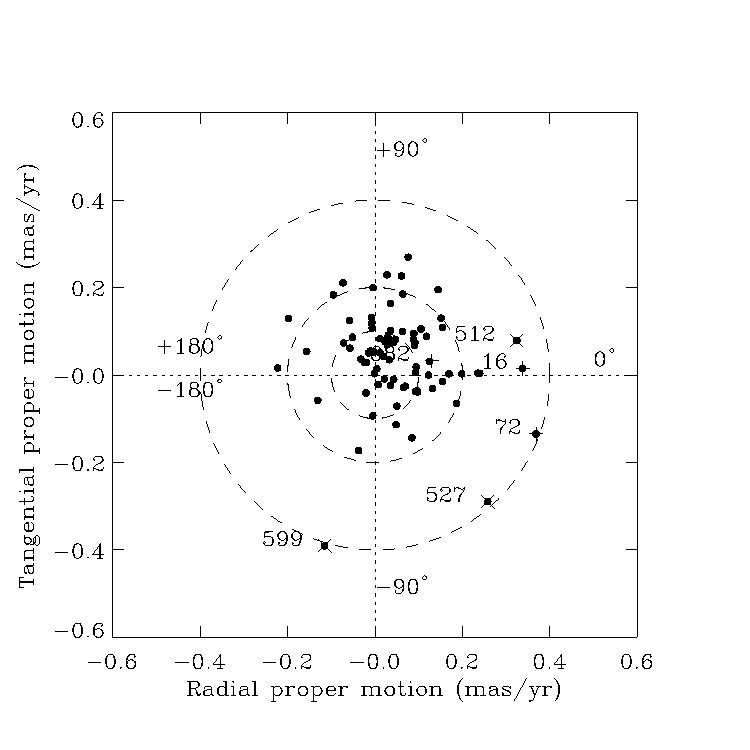
\includegraphics[width=0.5\textwidth]{figures/figure_polar_682-1.pdf}
  \caption{Polar plot of the relative proper motion components for the stars
    defining our reference frame. VFTS682 is indicated by the plus sign, and
    other notable outliers (see \citet{lennon:18}) are also labeled. Concentric dashed-lines denote relative proper motions of
    0.1, 0.2, and 0.4$\,\mathrm{mas\ yr^{-1}}$. Positive angle
    indicate a tangential component pointing in the counterclockwise
    direction, with 0 degrees corresponding to proper motion pointing
    radially outward from R136.
}
  \label{fig:pm_polar}
\end{figure}



These can be converted into
the components of the relative transverse velocity $\delta v_\mathrm{RA}^{Gaia}=24\pm19\,\kms$,
$\delta v_\mathrm{DEC}^{Gaia}=20\pm23\,\kms$, assuming a distance of
50\,kpc. These can be converted in a projected two-dimensional
velocity of $31\pm21\kms$. % (we do not account for the uncertainty in the distance
% estimate when propagating errors).
The radial velocity from
\cite{bestenlehner:11} then gives the third component along
the line of sight, allowing us to calculate the three-dimensional
peculiar speed of the star:

\begin{equation}
  \label{eq:speed_around_Gaia}
  v_\mathrm{pec}^{Gaia} = \sqrt{\left(\delta v_\mathrm{RA}^{Gaia}\right)^2
    +\left(\delta v_\mathrm{DEC}^{Gaia}\right)^2+\left(\delta
      v_\mathrm{rad}^{VFTS}\right)^2} = 44 \pm 21
  \kms \ .
\end{equation}

Therefore, two completely independent measures of the proper motion of
VFTS 682 relative to the surrounding field, one from HST and one from
\emph{Gaia} DR2, yield values of the peculiar three-dimensional
velocity of VFTS 682 (\Eqref{eq:speed_around_HST} and
\Eqref{eq:speed_around_Gaia}, respectively) which would make it the most massive runaway star
known to date. However, the large errors on both the proper motion measures
require confirmation with future astrometric data. 

\subsection{Does it come from the R136 cluster?}
\label{sec:r136_origin}

The red arrow in \Figref{fig:main} shows the proper motion of VFTS 682
relative to the region, and the lighter red arrows show the possible
range of directions within the uncertainties in the measured proper
motion. It is clear that the most likely origin of the star is R136,
as suggested based on numerical N-body simulations by \cite{fujii:11}
and \cite{banerjee:12}.

We can therefore consider the kinematic age for this star assuming
that it originates from the cluster,
\todo{lennon: use pm for kin age and not kms}
\begin{equation}
  \label{eq:kin_age}
  \tau_\mathrm{kin} = \frac{d_\parallel}{v_\parallel} \simeq
  \frac{29\,\mathrm{pc}}{34\,\kms} \simeq 0.85\pm\,0.02\, \mathrm{Myr} \ \ ,
\end{equation}
where $d_\parallel =29$\,pc is the projected distance from VFTS 682 to
the core of R136 \citep[][]{bestenlehner:11}, $v_\parallel \equiv \sqrt{\left(\delta v_\mathrm{RA}\right)^2
    +\left(\delta v_\mathrm{DEC}\right)^2} =34\pm
1\,\kms$ is the speed of the star relative to the cluster projected on the sky, obtained
using the relative proper motion components calculated in
\Secref{sec:runaway}.% , and we use the approximation $1 \kms \simeq 1
% \mathrm{pc \ Myr^{-1}}$.
As in the rest of this study, we neglect for
simplicity the error on the distance estimates, which amounts to about
$\sim$$2.2\%$, and is negligible compared to other uncertainties.

The kinematic age $\tau_\mathrm{kin}$ is similar or smaller than the apparent age
of the star of $1.0\pm 0.2$\,Myr from \cite{schneider:18}, which
corroborates the idea that the star is the result of a dynamical
ejection. 

\begin{figure}[tbp]
  \centering
  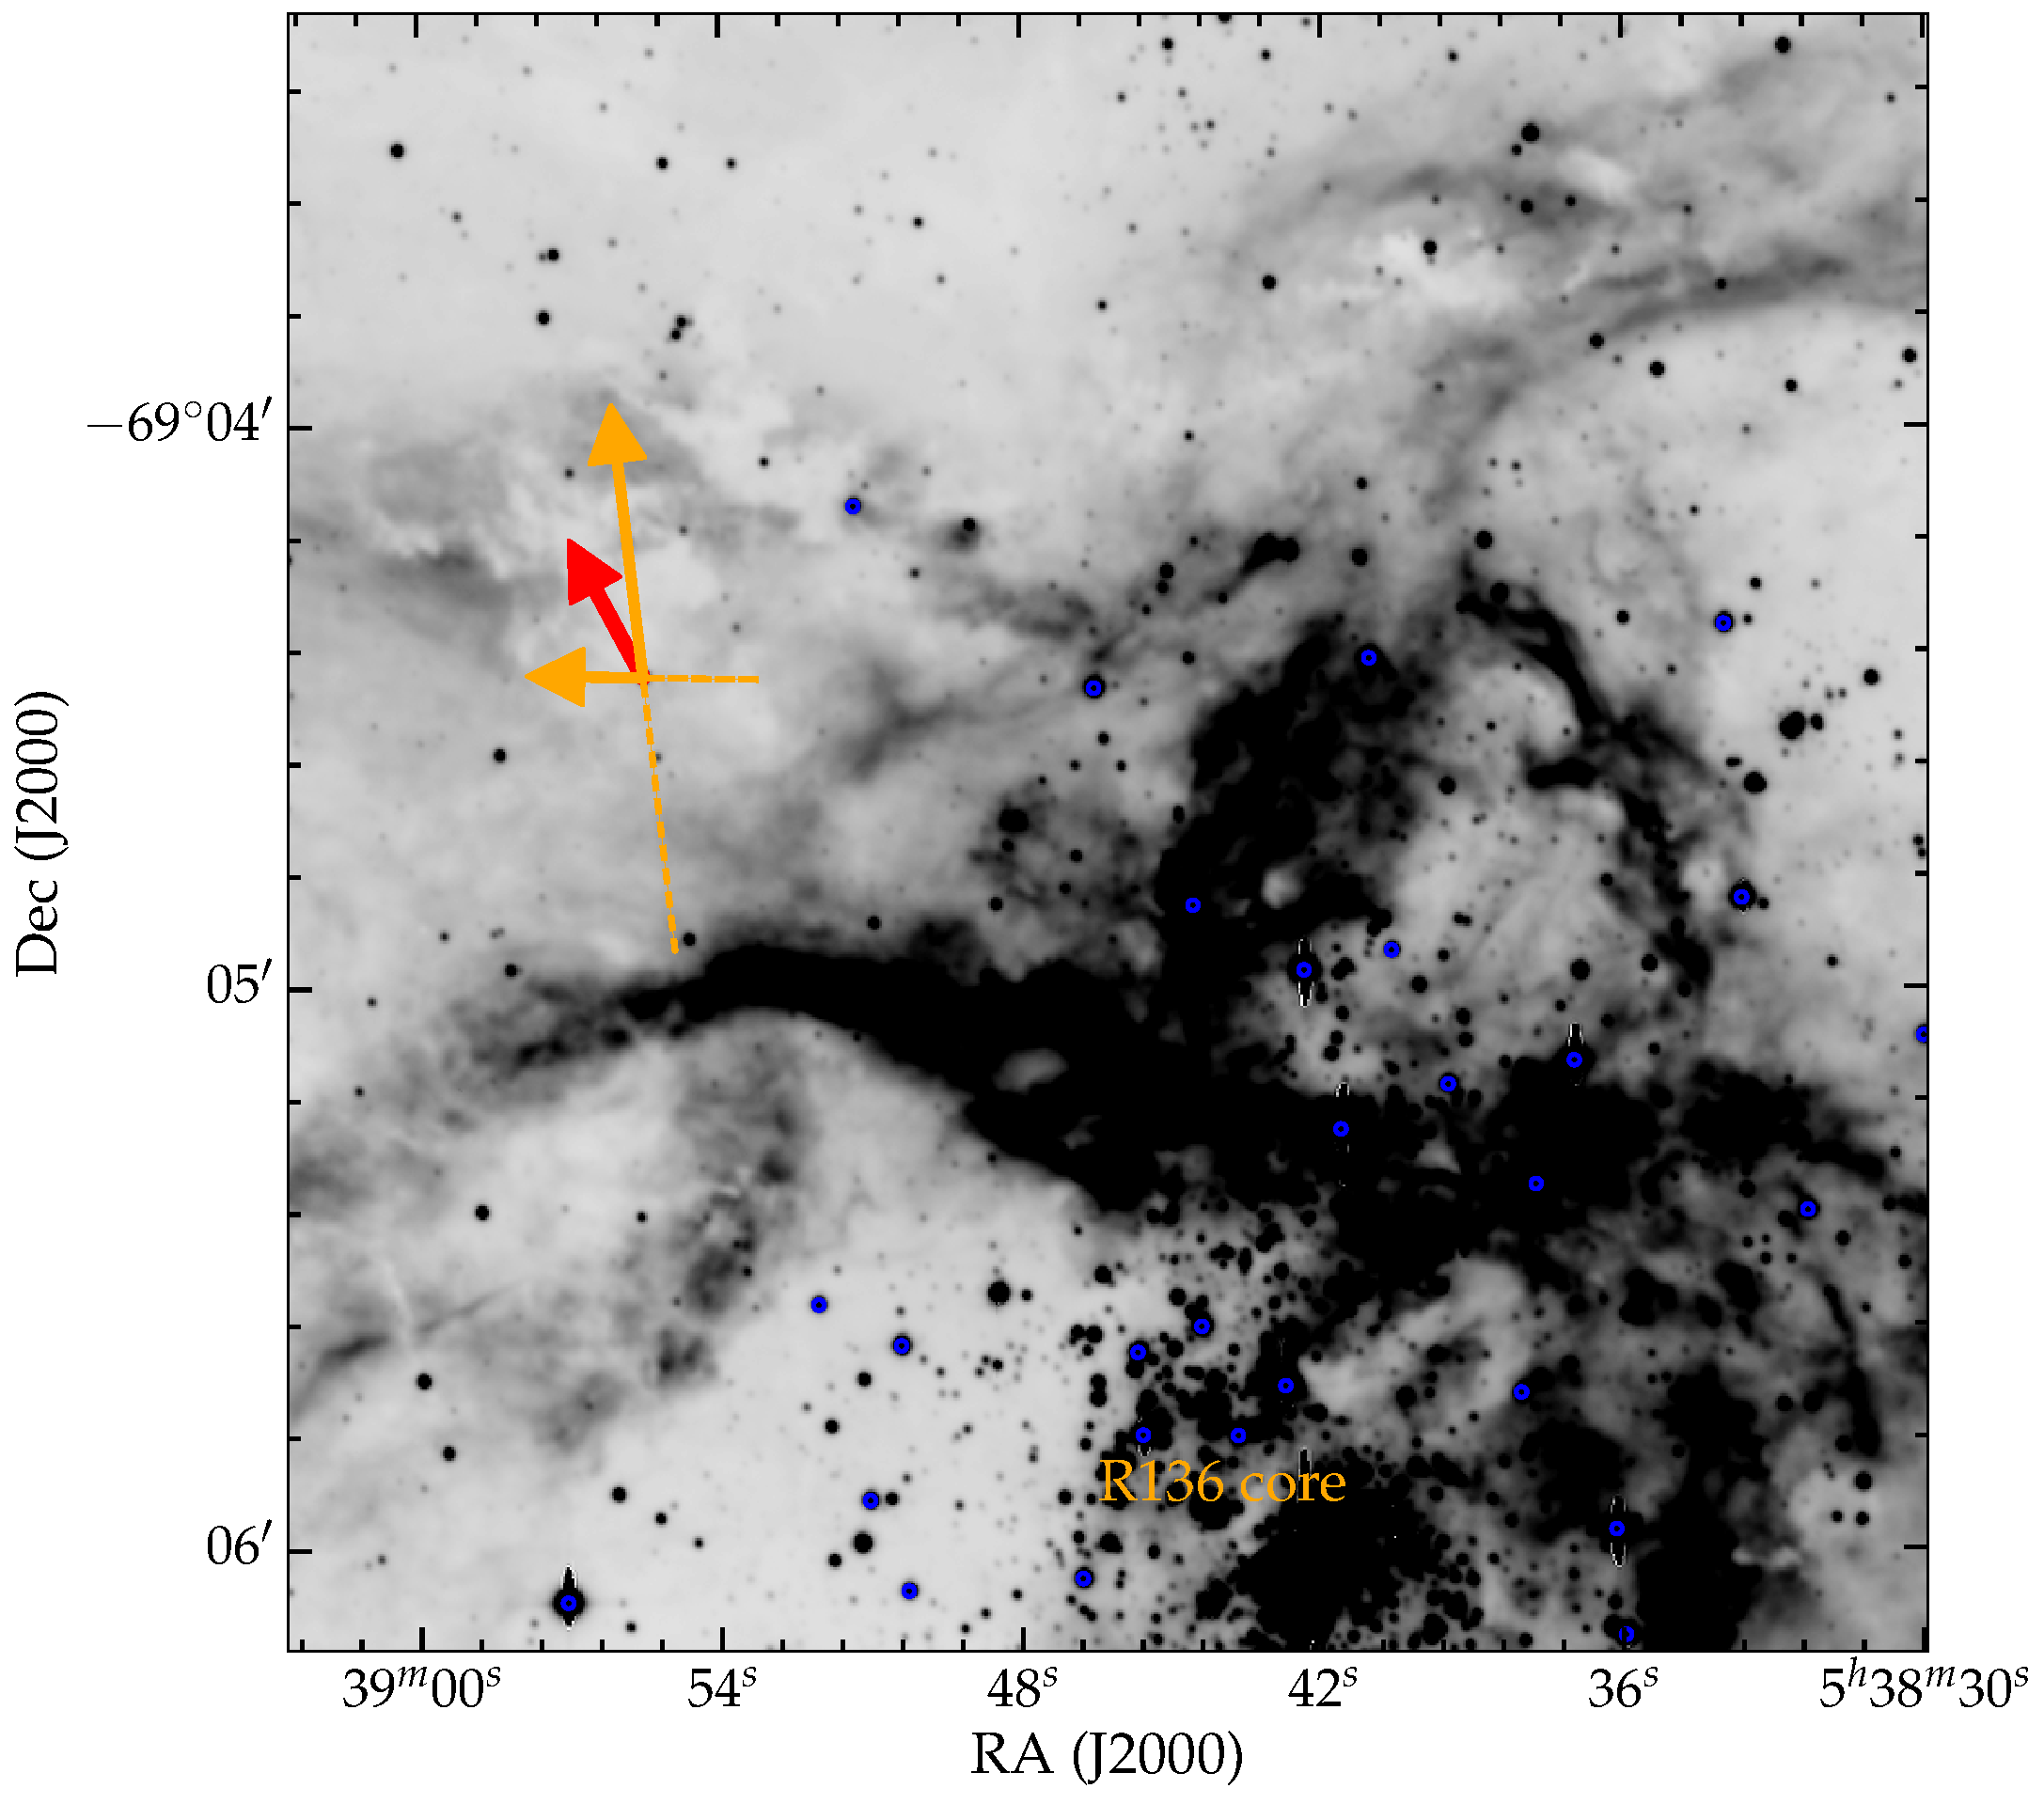
\includegraphics[width=0.48\textwidth]{./figures/main_plot_good}  
  \caption{The red solid arrow indicates the proper motion of VFTS 682
    relative to the region, starting from the present day position of
    the star. The orange arrows indicate the possible
    directions of projected motion within the errors, and are extended
    backwards (dashed) to illustrate the uncertainty on the origin of the
    star. The blue stars
    are a subset of those we use to define the local rest
    frame. \todo{load color picture on background}\todo{show
      separately arrows fro Gaia/HST and combination? Or show only
      combination? Right now it's Gaia only}}
  
  \label{fig:main}
\end{figure}


\section{Discussion}
\label{sec:discussion}
\todo{Selma: Should add caveat that it may be a spurious detection. That reconfirmation in following epochs is warranted. }

Based on our results, we claim that VFTS 682 is the most massive
runaway known to date, with a peculiar three-dimensional speed of $46\pm18\,\kms$. This means that isolated star formation is
\emph{not} required to explain this star. Its proper motion suggests that it was ejected from the cluster R136
$0.85\pm0.02$\,Myr ago. Because of the exceptionally large mass
of this star, this raises the question of which stars must populate
the core of the cluster.

Dynamical ejections due to N-body interactions typically (although, not necessarily) eject the least
massive star among those interacting \cite[e.g.,][]{banerjee:12}. This means that, just
based on the kinematic properties of VFTS 682, we would expect several
stars with initial masses larger than $\sim$$150\,M_\odot$ in the
cluster R136.
This is consistent with the detection
of extremely massive stars by \cite{crowther:10} in the core of the
cluster. The projected rotational equatorial
velocity\footnote{However, the determination of the rotational
  velocity for stars showing lines in emission is complicated by the optically thick wind screening the surface of the star, and should be
  considered with caution.} of VFTS 682
reported by \cite{schneider:18} is $v\sin(i)<200\,\kms$, which is in
line with the average rotation rate of massive stars in the region
\citep[][]{ramirez-agudelo:15}. This suggests that VFTS 682 (i) has not
experienced rotationally induced chemically homogeneous evolution
\citep[][]{maeder:00,demink:09,marchant:16}, and (ii) it has not
accreted mass from or merged with a binary companion, nor will it, since the multi-epoch
data of the VFTS survey rule out the presence of a close companion at the
present day. Moreover, the spectral type of VFTS 682
\citep[WNh5,][]{bestenlehner:11} is the same as R136a1-a3, i.e.~the
three most massive stars detected in the core of the cluster by
\cite{dekoter:97,crowther:10,crowther:16}, with an astonishing similarity in particular with
the spectrum of R136a3. Therefore,
VFTS 682 might be an ideal target to constrain the stellar physics of
stars with masses well above $\sim$$100\,M_\odot$: its isolation makes
it an easier target for observations compared to the similar stars
present in the crowded core of R136.

\citet{banerjee:12} used N-body simulations of fully segregated
clusters with all massive stars in binaries to suggest that VFTS 682
was ejected from R136. They
demonstrated that the cluster potential does not significantly change
the velocity of the star after the ejection. In their
model, they relied on (dynamically driven) stellar mergers to explain the high masses of
VFTS 682 and the massive members of R136. While it is not possible to
robustly exclude that VFTS 682 is itself a merger, as already
mentioned, its spectrum does not show any of the obvious signatures
like fast rotation. To eject such a massive object, the cluster is
expected to have produced
a large number of massive runaways. Indeed, several relatively
isolated massive stars are observed in the region, some with known
large radial velocities. A comprehensive study of the kinematic
properties of all the massive stars surrounding R136 might shed light
on whether some can be unequivocally identified as merger products. It
is also possible that the star or binary that caused the ejection of
VFTS 682 might have been ejected in the opposite direction, and is also
in isolation at present day. 


The similarities between VFTS 682 and the WNh5 stars in the core of
R136 are also in agreement with the ``bully binary'' model of
\cite{fujii:11}. Based on their numerical results, they suggested that
early in the evolution of a cluster, dynamical interactions form an extremely
massive binary, which then tightens its orbit by ejecting other stars passing
by. Interpreting our results for VFTS 682 through the lens of their simulations
suggests the presence of a close binary with total mass
$M_1+M_2\gtrsim 300\,M_\odot$ in the core of the cluster. Such bully
binary could be R145 according to \cite{fujii:11}, and it might be an
ideal observational candidate for a dynamically formed progenitor system of
a binary black-hole, provided that stars this massive can avoid a
pair-instability supernova \cite[][]{fowler:64, rakavy:67} at LMC
metallicity \citep[see also][]{langer:07}. Similarly, the final fate of VFTS 682 could be either a
pair-instability supernova without compact remnant formation, or
possibly direct collapse to a black hole above the $2^\mathrm{nd}$
mass gap. The amount of mass loss of these stars will determine their final core
mass and thus their final fate.

The kinematic age of VFTS 682 puts an
upper limit to the timescale to form the ``bully binary'' in
R136. The cluster must have been at the very beginning of its
evolution, given the age estimate of $\lesssim 2$\,Myr
\citep[][]{crowther:10,sabbi:12} and the kinematic age of VFTS 682. If the
cluster is indeed younger than the shortest stellar lifetime
\citep[$\sim$3\,Myr, e.g.,][]{brott:11, zapartas:17}, then the alternative
explanation for ejection of VFTS 682 from the disruption of a binary
by a core-collapse event is excluded since the region is too young for stars
to have experienced core-collapse already.
 
The variability of VFTS 682, reminiscent of LBV stars, suggests
that VFTS 682 (and therefore its analogs in the core of R136) might
experience enhanced mass loss episodes in LBV eruptions. \citet{smith:15} made the highly
debated\footnote{See, e.g., \cite{humphreys:16, davidson:16, smith:16}.}
claim that LBV stars are typically isolated form O-type stars. The fact that VFTS 682 is a dynamically
ejected runaway which might evolve into an LBV star suggests that
N-body interactions also play a role in explaining the apparent
isolation of at least some LBV stars. 

\citet{lennon:18} carried out a study similar to ours on VFTS16, another
massive star ($\sim$$90\,M_\odot$) in the 30 Doradus region, previously
known to be a runaway from the value of
its radial velocity. They also concluded that VFTS16 is 
the result of a dynamical ejection from the R136 cluster. 
The value of $\tau_\mathrm{kin}\simeq0.85$\,Myr we find for VFTS 682 (see \Secref{sec:r136_origin}) is smaller
than the corresponding value for VFTS16: \cite{lennon:18} inferred a kinematic age of
$\sim$1.5\,Myr, possibly in tension with the apparent age of that star. This means that the more
massive VFTS 682 was ejected later than VFTS16 from the same cluster.

The numerical simulations from \cite{oh:16} suggest that dynamical
interaction eject the majority of the stars during or shortly after the cluster
core-collapse. The large number of isolated massive stars around it
suggest that R136 has already evolved past the
time of maximum stellar density. This might have implications for the
question on whether the cluster formed via a monolithic collapse, or
as a (potentially ongoing) merger of several sub-clusters.

\citet{oh:16} also showed that the mass and velocity distribution of the ejected star depends on the cluster initial conditions
(whether it is segregated, its primordial binary fraction and initial period
distribution of the binary population), therefore studies on
the population of isolated massive stars in the surroundings of R136
might shed light on its initial stellar population and dynamical
state. 

VFTS 682 is the most massive runaway known to date, and its ejection
from the cluster R136 likely implies that it is only the ``tip of the
iceberg'' of possibly extremely massive runaways in the
region. Studies of this population, enabled by recent HST and \emph{Gaia} observations will put constraints on the evolution
of these extreme stars, together with the formation and evolution of
the central cluster itself.

\bibliographystyle{aa}
\bibliography{bibliography/vfts682}

\begin{acknowledgements}
  \small
  We are grateful to S.~Torres for 
  very useful discussions on the
  \emph{Gaia} DR2 dataset, and to M.~C.~Ramirez-Tannus for invaluable help.
  SdM has received funding under the European Unions Horizon 2020 research and innovation programme from the European Research
  Council (ERC) (Grant agreement No. 715063). VHB acknowledges support from the NRC-Canada Plaskett Fellowship.
  This work has made use of data from the ESA space mission \emph{Gaia} (\url{http://www.cosmos.esa.int/gaia}), processed by the \emph{Gaia} Data Processing and Analysis Consortium (DPAC, \url{http://www.cosmos.esa.int/web/gaia/dpac/consortium}). Funding for the DPAC has been provided by national institutions, in particular the institutions participating in the \emph{Gaia} Multilateral Agreement. 
  The background image of \Figref{fig:main} is based on observations
  made with ESO Telescopes at the La Silla Observatory under programme
  ID 076.C-0888, processed and released by the ESO VOS/ADP group.
  This research made use of APLpy, an open-source plotting package for Python \citep[][]{robitaille:12}.
\end{acknowledgements}

\end{document}




%%% Local Variables:
%%% mode: latex
%%% TeX-master: t
%%% End:
